\chapter{Espacios vectoriales}

\section{Espacios vectoriales de funciones}
\label{subsection: espacios vect de funciones}

Sean $X \neq \emptyset$ un conjunto no vacío cualquiera
y $(F, +, 0, \cdot, 1)$ un campo. Consideremos al conjunto
\[
F^{X} := \{ f: X \longrightarrow F :
\hspace{0.2cm} f \textit{ es función} \} 
\]
de funciones de $X$ en $F$; aprovechando la estructura de campo
en $F$, vamos a dotar al conjunto $F^{X}$ de estructura
de $F-$espacio vectorial.\\

\begin{itemize}
	\item \textbf{Definición de suma de funciones:}
	Definimos a la operación binaria suma
	\begin{equation}
		\label{eq: suma de funciones}
		\hat{+} : F^{X} \times F^{X} \longrightarrow F^{X}
	\end{equation}
	como sigue: dadas $f, g \in F^{X}$ cualesquiera, 
	la función $f \hat{+} g \in F^{X}$ se define puntualmente como
	\begin{equation}
		\label{eq: suma funciones puntual}
	(f \hat{+} g)(x) = f(x) + g (x), \hspace{0.2cm}
	x \in X.
	\end{equation}
	Nota que, en la ecuación anterior, el signo $\hat{+}$
	que aparece a la izquierda es la operación binaria
	que estamos definiendo en \eqref{eq: suma de funciones}, 
	mientras que el signo $+$ de la derecha es la suma
	del campo $F$: \textit{a partir de la operación
	suma en $F$ estamos diciendo cómo sumar elementos
	de $F^{X}$}.
	
	\item \textbf{Definición de producto por escalares:}
	Definimos a un producto por escalares
	\begin{equation}
		\label{eq: producto por escalares}
	\star : F \times F^{X} \longrightarrow F^{X} 	
	\end{equation}		
	como sigue: si $a \in F$ y $f \in F^{X}$, la función
	$a \star f \in F^{X}$ se define puntualmente como
	\begin{equation}
		\label{eq: definicion prod esc}
	(a \star f)(x) = a f(x), \hspace{0.2cm}
	x \in X.
	\end{equation}
	Nota cómo estamos usando la operación producto
	del campo para definir el producto por escalares.
	
	\item \textbf{Neutro aditivo:} Proponemos como 
	neutro para la operación suma de funciones (c.f. \eqref{eq: suma de funciones}) a la función $\hat{0} : X \longrightarrow F$
	definida como sigue:
	\begin{equation}
		\label{eq: funcion cero}
		\hat{0}(x) = 0, \hspace{0.2cm} x \in X,
	\end{equation}
	es decir, a la función que mapea todo punto
	de $X$ al neutro aditivo del campo $F$.
\end{itemize}

Demostremos que 
$(F^{X}, \hat{+}, \star)$
es un $F-$espacio vectorial.\\


En lo que sigue, vamos a demostrar igualdades que tienen lugar
en $F^{X}$, es decir, igualdades entre funciones.
Recuerda que dos funciones son iguales si tienen el mismo dominio,
codominio y misma regla de correspondencia: puesto que todos los 
elementos de $F^{X}$ tienen dominio $X$ y codominio $F$, para
demostrar que $f, g \in F^{X}$ son iguales basta ver que
\[
f(x) = g (x) \hspace{0.2cm}
\textit{ para toda } x \in X.
\]

\begin{enumerate}
	\item \textbf{Asociatividad de $\hat{+}$:}
	sean $f, g, h \in F^{X}$. Mostremos que 
	\[
	(f \hat{+} g) \hat{+} h = f \hat{+} ( g \hat{+} h).
	\]
	Sea $x \in X$.
	Usando la definición de suma de funciones dada en 
	\eqref{eq: suma funciones puntual},
	tenemos que 
	\begin{align*}
	((f \hat{+} g) \hat{+} h )(x) = &
	(f \hat{+} g)(x) + h(x)
	= (f(x) + g(x)) + h(x) \\
	= & f(x) + (g(x) + h(x)) = f(x) + (g \hat{+} h)(x) \\
	= & (f \hat{+} (g \hat{+} h)) (x).
	\end{align*}
	La tercera igualdad se da porque la suma en $F$
	es asociativa.
	
	\item \textbf{Elemento neutro para la suma:}
	Si $f \in F^{X}$ cualquiera, veamos que
	\[
	\hat{0} \hat{+} f = f = f \hat{+} \hat{0}.
	\]
	Probemos la primera igualdad; la otra se tiene de forma 
	análoga. Usaremos la definición 
	\eqref{eq: funcion cero}
	de la función cero $\hat{0}$ y la definición de suma de funciones dada en 
	\eqref{eq: suma funciones puntual}.
	Para toda $x \in X$,
	\[
	(\hat{0} \hat{+} f) (x) = 
	\hat{0}(x) + f(x) = 0 + f(x) = f(x).
	\]
	
	\item \textbf{Existencia de inversos aditivos:}
	\hlgray{Ejercicio:} Dada una función $f \in F^{X}$, propón
	una función $g \in F^{X}$ que sea el neutro
	aditivo de $f$, es decir, una función tal que
	\[
	f \hat{+} g = \hat{0} = g \hat{+} f.
	\]
	Sugerencia: Defínela puntualmente, usa la existencia
	de inversos aditivos en el campo $F$.
	Naturalmente, a tal función $g$ la denotaremos por $-f$.
	
	\item \textbf{Conmutatividad de $\hat{+}$}:
	\hlgray{Ejercicio:} Demuestra que la suma de funciones
	es conmutativa, es decir, que dadas cualesquiera
	$f, g \in F^{X}$, 
	\[
	f \hat{+} g = g \hat{+} f.
	\]
	
	\item \textbf{(EV-5)} Sea $f \in F^{X}$ cualquiera;
	es fácil ver que ocurre
	\[
	1 \star f = f
	\]
	pues, según la definición del producto por escalares dada en 
	\eqref{eq: definicion prod esc}, 
	para toda $x \in X$ se tiene que
	\[
	(1 \star f)(x) = 1 f(x) = f(x).
	\]
	\item \textbf{(EV-6)} Si $a, b \in F$
	y $f \in F^{X}$, demostremos que
	\[
	(ab) \star f = a \star (b \star f).
	\] 
	Sea $x \in X$.
	\[
	((ab) \star f)(x) = ab f(x) = a (bf(x))
	= a ((b \star f)(x)) = (a \star (b \star (f)))(x).
	\]
	\item \textbf{(EV-7)}
	\hlgray{Ejercicio: } Demuestra que,
	para todo $a \in F$ y cualesquiera
	$f, g \in F^{X}$, 
	\[
	a \star (f \hat{+} g) = a \star f \hat{+} a \star g.
	\]
	
	\item \textbf{(EV-8)}
	\hlgray{Ejercicio: } Demuestra que,
	para toda $f \in F^{X}$ y cualesquiera
	$a, b \in F$, 
	\[
	(a + b) \star f = a \star f \hat{+} b \star f.
	\]
	
\end{enumerate}

\begin{ejem}
Si $\mathcal{C}(\IR) = \{ f: \IR \longrightarrow \IR :
\hspace{0.2cm} f \textit{ es continua} \}$,
es claro que 
$\mathcal{C}(\IR) \subseteq \IR^{\IR}$.
\end{ejem}


\subsubsection{Espacio de funciones de soporte finito $F^{(X)}$}


\begin{defi}
Sean $X \neq \emptyset$ un conjunto, $F$ un campo. Dada
$f: X \longrightarrow F$ función (i.e. un elemento
de $F^{X}$), definimos su \textbf{soporte}
\begin{marginfigure}
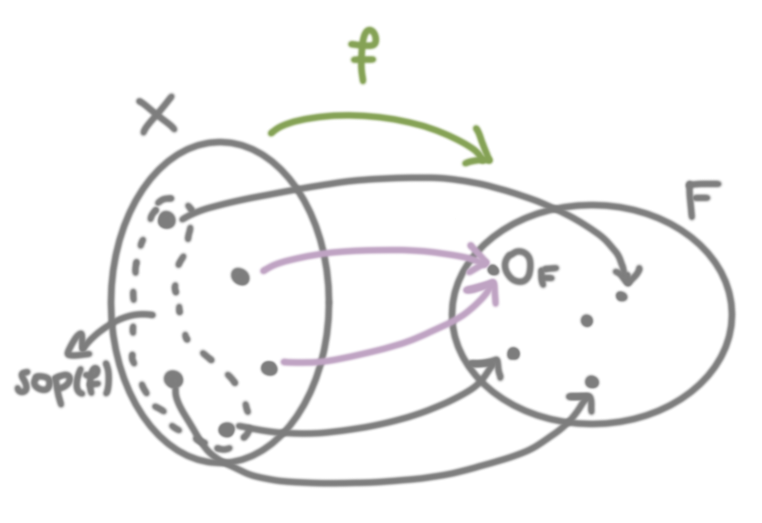
\includegraphics[scale= 1.3]{ 1} 
		\caption{Representación gráfica del soporte de una función.}
\end{marginfigure}
como el conjunto de los puntos del dominio para 
los que $f$ no se anula:
\[
sop(f) :=
\{ x \in X  | \hspace{0.2cm} f(x) \neq 0 \}.
\]

\end{defi}

\begin{ejem}
Tomemos a $X = \IN$. Acostumbramos llamar a los 
elementos de $F^{\IN}$ \textbf{sucesiones en $F$}.
De hecho, dada una función $f \in F^{\IN}$, 
es usual identificarla con el conjunto de sus imágenes:
\[
f = (f_{n})_{n \in \IN}, 
\hspace{0.2cm} \textit{ donde }
f_{n} := f(n).
\]
\hlgray{Ejercicio:} Demuestre que,
si $f = (f_{n})_{n \in \IN} \in F ^{\IN}$ tiene soporte 
finito, entonces $\lim_{n \rightarrow \infty} f(n) = 0$.
¿Se vale la otra implicación?
\diam
\end{ejem}


\begin{defi}
Denotaremos por $F^{(X)}$ al conjunto de las funciones
de $X$ en $F$ que tienen soporte finito, es decir,
\[F^{(X)} := \{ f \in F^{X}  | \hspace{0.2cm}  
|sop(f) < \infty|\}.
\]
\end{defi}


Para lo que sigue, necesitamos que el lector recuerde
(o al menos esté de acuerdo en aceptar como ciertos)
los siguientes hechos:
\begin{itemize}
	\item La cardinalidad del conjunto vacío es $0$.
	El conjunto vacío es el único conjunto de cardinalidad $0$.
	\item Si $A$ y $B$ son dos conjuntos finitos, entonces
	$A \cup B$ es también finito.
	\item Si $A$ está contenido en $B$ y $B$ es finito, entonces
	$A$ también lo es.
\end{itemize}

\begin{prop}
Si $X \neq \emptyset$ y $F$ es un campo, entonces
$F^{(X)}$ es un subespacio de $F^{X}$.
\end{prop}
\noindent
\textbf{Demostración.}
Usemos los criterios dados en la proposición $(*-sub)$
para mostrar que $F^{(X)} \leq F^{X}$.
\begin{enumerate}
	\item Si $\hat{0}: X \longrightarrow F$ es la función
	cero, 
	\[
	sop(\hat{0}) = \{ x \in X  | \hspace{0.2cm} \hat{0}(x) \neq 0\}
	= \emptyset,
	\]
	luego, $\hat{0}$ tiene soporte finito, o sea, 
	$\hat{0} \in F^{(X)}$.
	
	\item Sean $f, g \in F^{(X)}$; veamos que $f + g \in F^{(X)}$.
	Es decir, usando que $f$ y $g$ tienen soporte finito, mostremos
	que $f+g$ también tiene soporte finito.
	Si $sop(f + g) = \emptyset$, acabamos. Supongamos ahora
	que $sop(f+g) \neq \emptyset$. Note que, si 
	$x \in sop(f+g)$, entonces
	\[
	f(x) + g(x) = (f+g)(x) \neq 0,
	\]	
	luego, no ocurre $f(x) = 0 = g(x)$, es decir,
	\[
	x \not\in (sop(f))^{c} \cap (sop(g))^{c},
	\]
	o sea, 
	\[
	x \in sop(f) \cup sop(g).
	\]
	Con esto demostramos la contención
	\[
	sop(f+g) \subseteq sop(f) \cup sop(g).
	\]
	Como $sop(f)$ y $sop(g)$ son, por hipótesis, ambos
	finitos, su unión también lo es, luego
	$sop(f+g)$, por ser subconjunto de un conjunto finito,
	es finito.
	
	\item Sean $f \in F^{(x)}$ y $a \in F$; probemos que
	$af \in F^{(X)}$. Si $a = 0$, 
	$a f = \hat{0} \in F^{(X)}$; supongamos ahora $a \neq 0$.
	\marginnote{Recuerda que, en un campo, el producto de dos
	elementos es cero si y sólo si al menos uno de los dos es cero.}
	Entonces,
	\begin{align*}
	x \in sop(af) & \Leftrightarrow  af(x) \neq 0 \\
	& \Leftrightarrow  a \neq 0 \textit{ y } f(x) \neq 0 \\
	& \Leftrightarrow  f(x) \neq 0 
	\Leftrightarrow x \in sop(f).
	\end{align*}
	Así, $sop(a f) = sop(f)$, luego, $af$ tiene, al igual
	que $f$, soporte finito.
\end{enumerate}

\QEDB
\vspace{0.2cm}

\section{El subespacio generado por un subconjunto y suma de subespacios}


Dado $V$ un $F-$espacio vectorial, 
sea $\{ W_{\alpha} \}_{\alpha \in I}$ una familia no vacía de subespacios
de $V$. A partir de esta familia, ¿cómo podemos construir otro
subespacio de $V$?
Consideremos a la unión e intersección de la familia, o sea,
a los conjuntos

\begin{equation}
	\label{eq: int fam subesp}
	\bigcap_{\alpha \in I} W_{\alpha} :=
\{ x \in V  | \hspace{0.2cm} x \in W_{\alpha} \textit{ para toda }
\alpha \in I  \} \subseteq V,
\end{equation}
y
\begin{equation}
	\label{eq: union fam subesp}
	\bigcup_{\alpha \in I} W_{\alpha} :=
\{ x \in V  | \hspace{0.2cm} x \in W_{\alpha} \textit{ para algúna }
\alpha \in I  \} \subseteq V.
\end{equation}

¿Son estos subespacios de $V$?
Tenemos una
respuesta afirmativa y otra negativa.

\begin{prop}
La intersección \eqref{eq: int fam subesp} de la familia
de subespacios $\{ W_{\alpha} \}_{\alpha \in I}$
de $V$ es un subespacio de $V$.
\end{prop}
\noindent
\textbf{Demostración.}
\begin{itemize}
	\item[i)] Puesto que el cero es elemento de \textit{todo}
	subespacio de $V$, claro que $0 \in W_{\alpha}$ para
	toda $\alpha \in I$, luego, $0 \in \bigcap_{\alpha \in I} W_{\alpha}$
	\item[ii, iii)] Sean $x, y \in \bigcap_{\alpha \in I} W_{\alpha}$,
	$a \in F$; claro que 
	$x+y, ax \in \bigcap_{\alpha \in I} W_{\alpha}$
	pues, dado $\alpha \in I$ un índice cualquiera,
	$x, y \in W_{\alpha}$, luego, como 
	$W_{\alpha}$ es subespacio de $V$, $x+y, ax \in W_{\alpha}$.
\end{itemize}

\QEDB
\vspace{0.2cm}

La demostración anterior fue muy sencilla pues, para
que un vector sea elemento de la intersección
$\bigcap_{\alpha \in I} W_{\alpha}$,
debe estar en \textit{todos} los elementos de la familia a la 
vez, y todos los $W_{\alpha}$ cumplen  
los tres puntos de la proposición (*-sub).
La condición que debe cumplir un vector para estár en la 
unión de la familia es mucho más laxa; es necesario y suficiente
que sea elemento de un solo miembro de la familia
$\{ W_{\alpha} \}_{\alpha \in I}$.
Dados
$x, y \in \bigcup_{\alpha \in I} W_{\alpha}$,
existen $\alpha_{1}, \alpha_{2} \in I$
tales que $x \in W_{\alpha_{1}}$ y 
$y \in W_{\alpha_{2}}$. Nota que \textit{no podemos
decir que $x$ y $y$ son elementos de un mismo subespacio}, luego,
esta información no parece implicar que la suma sea elemento de la 
unión.


\begin{ejem}
(Que muestra que la unión de subespacios puede no ser un subespacio).
Sea $(a, b) \subseteq \IR$ un intervalo abierto cualquiera.
Considere al $\IR-$espacio vectorial
\[
\IR^{(a, b)} = \{ f: (a, b) \longrightarrow
\IR  | \hspace{0.2cm} f \textit{ es función.} \}
\]

Sean 
\[
\mathcal{B}_{a, b} = \{ f \in \IR^{(a, b)}  | \hspace{0.2cm}
f \textit{ es acotada}  \}, \hspace{0.4cm}
\mathcal{C}_{a, b} = \{ f \in \IR^{(a, b)}  | \hspace{0.2cm}
f \textit{ es continua}  \}.
\]
Como sabes por tus cursos de cálculo, estos son subespacios
de $\IR^{(a, b)}$. En la imagen se muestran la gráfica
de una función continua $f$ y una acotada
$g$ en $(a, b)$ para las que la suma no es ni continua ni 
acotada (i.e. tales que $f, g \in \mathcal{B}_{a, b} \cup
\mathcal{C}_{a, b}$ pero $f + g \not\in \mathcal{B}_{a, b}
\cup \mathcal{C}_{a, b}$). 
\begin{figure}[H]
	\sidecaption{
	Con el sumando continuo rompemos la acotación, y con
el sumando acotado, la continuidad.
	\label{fig: 2}
	}
	\centering
	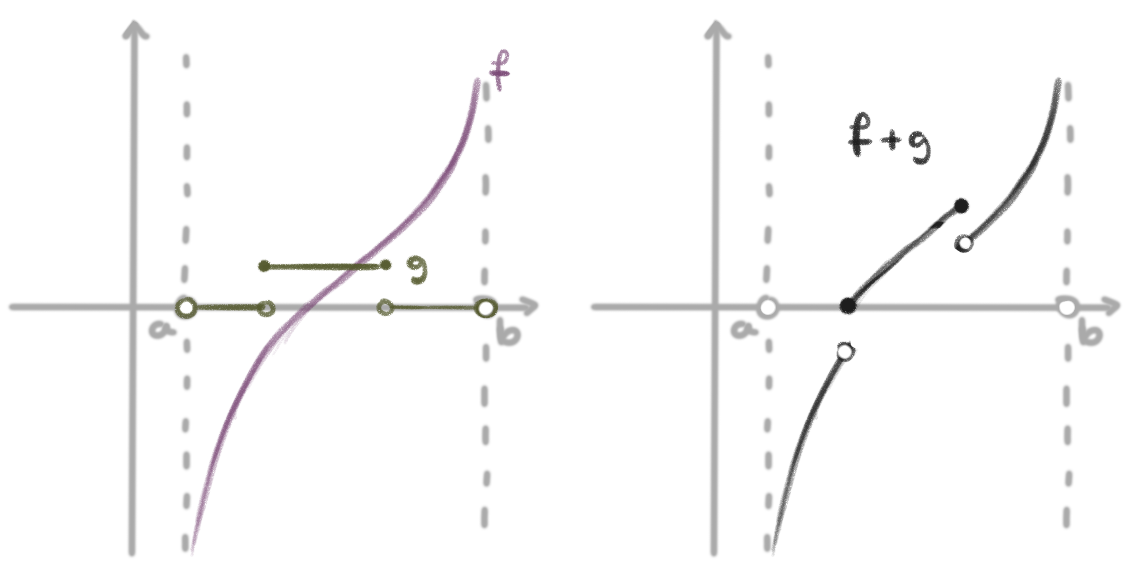
\includegraphics[scale = 2.5]{2} 
\end{figure}	
\diam
\end{ejem}

\hlgray{Ejercicio:} Si $\{ W_{\alpha} \}_{\alpha \in I}$
es una colección de subespacios de $V$ tal que
\[
(\forall i, j \in I)(\exists k \in I): \hspace{0.2cm}
W_{i}, W_{j} \subseteq W_{k},
\]
entonces $\bigcup_{\alpha \in I} W_{\alpha}$ es un subespacio de $V$.


 \begin{center}
 --- * * * ---
 \end{center}
Ahora, dado $V$ un $F-$espacio vectorial, a veces nos interesará
limitarnos a trabajar no con todo el espacio $V$, sino con un 
subconjunto $X$ de este. Como también queremos aprovechar
la estructura algebráica, nos interesará que tal colección $X$
sea, más que subconjunto, subespacio de $V$.
Esto puede ocurrir o no: lo que siempre podemos hacer
es considerar a la familia $\{ W \leq V : 
\hspace{0.2cm} X \subseteq W \}$ de subespacios más pequeños
(en el sentido que están propiamente contenidos en $V$)
que contienen a nuestro conjunto de interés de $X$, y 
``condensar'' a esta familia via su intersección.

\begin{defi}
Sean $V$ un $F-$espacio vectorial, $X \subseteq V$. 
El subespacio
\begin{equation}
	\label{eq: sub generado por X}
	\langle X \rangle := \bigcap \{ W \leq V : \hspace{0.2cm}
	X \subseteq W \},
\end{equation}
o sea, la intersección de la familia de todos los subespacios
de $V$ que contienen a $X$, es llamado el 
\textbf{subespacio de $V$ generado por $X$}.
\end{defi}

\begin{prop}
$\langle X \rangle$ es el menor subespacio de $V$
que contiene a $X$, es decir,
\marginnote{Estamos considerando a la contención de conjuntos
como orden; el que un conjunto $A$ sea menor que un conjunto
$B$ significa que $A$ está contenido en $B$.}
\[
\forall \hspace{0.1cm} W \leq V: \hspace{0.2cm}
X \subseteq W \Rightarrow \langle X \rangle \leq W.
\]
\end{prop}
\noindent
\textbf{Demostración.}
Es clara pues, $\langle X \rangle$, al ser por definición
la intersección de la familia de subespacios que
contienen a $X$, está contenido en cada uno de sus integrantes.

\QEDB
\vspace{0.2cm}

En resumen: si $X$ no es subespacio, siempre podemos
considerar a $\langle X \rangle$, \textit{el menor}
subespacio de $V$ que contiene al conjunto de interés.

\hlgray{Ejercicio:} Demuestre que, si $X \leq V$,
entonces $X = \langle X \rangle$.

\begin{obs}
Por definición,
$\langle \emptyset \rangle $ es la intersección 
de la familia de subespacios que contienen a 
$\emptyset$ - o sea, es la intersección de todos los subespacios
de $V$. Como $\{ 0 \}$ es el menor subespacio de $V$, concluimos que
\[
\langle \emptyset \rangle = \{ 0 \}.
\] 
\end{obs}

En \eqref{eq: sub generado por X} decimos cómo
construir a tal $\langle X \rangle$; el objetivo ahora es dar
una descripción completa de sus elementos, es decir,
dar un criterio concreto en base al cual determinar
cuándo un vector $x$ del espacio pertenece a 
$\langle X \rangle$.

Según la proposición (*-sub), $X$ puede no ser subespacio
por cumplirse al menos una de las tres razones siguientes:
\begin{itemize}
	\item $\hat{0} \not\in X$; corregimos esto agregando
	al vector cero.
	\item Existen $x, y \in X$ tales que 
	$x+y \not\in X$; esto se puede arreglar agregando
	sumas de elementos de $X$.
	\item Existen $a \in F$ y $x \in X$ para los que
	$ax \not\in X$. Para que esto no ocurra, podemos 
	agregar los múltiplos escalares de los elementos de $X$.
\end{itemize}

Parece que el problema de no ser subespacio se arregla
si agregamos sumas finitas de múltiplos escalares de elementos
de $X$ (pues así estamos forzando a que los tres puntos de la 
proposición (*-sub) ocurran). Demos un nombre a tales
sumas de elementos de $X$.

\begin{defi}
Sea $V$ un $F-$espacio vectorial, $X \subseteq V$. Una 
\textbf{combinación lineal} en $V$ de elementos de $X$ es cualquier
vector de la forma
\[
\sum_{i=1}^{n} a_{i}x_{i},
\hspace{0.2cm} \textit{ con }
n \geq 1 \textit{ entero, }
x_{i} \in X, a_{i} \in F
\textit{ para toda } 1 \leq i \leq n.
\] 
\end{defi}

Según la discusión anterior, parece que para ``extender''
a $X$ a un subespacio de la forma mínima, hay que agregar
todas las combinaciones lineales de elementos de $X$, pues con esto
parece quedar asegurada la cerradura bajo suma y multiplicación
por escalares. Confirmamos nuestras sospechas con el siguiente resultado.

\begin{prop}
	\label{prop: caract elementos del subesp generado por X}
Si $\emptyset \neq X \subseteq V$, entonces
$\langle X \rangle$ consta de todas las combinaciones lineales
de elementos de $X$, es decir,
\begin{equation}
	\label{eq: elementos del generado de X}
\langle X \rangle = \left\{ \sum_{i=1}^{n} a_{i}x_{i} | \hspace{0.2cm} 
n \in \IN, x_{i} \in X, a_{i} \in F \hspace{0.2cm} \textit{ para toda }
1 \leq i \leq n \right\}
\end{equation}
\end{prop}
\marginnote{En inglés, al conjunto de la derecha en 
\eqref{eq: elementos del generado de X} se le conoce como
el ``span'' de $X$. La proposición 
\ref{prop: caract elementos del subesp generado por X}
nos dice que el span de un conjunto $X$ es el menor subespacio
que contiene a $X$.}
\noindent
\textbf{Demostración.}
Sea 
\[
\mathcal{A} = \left\{ \sum_{i=1}^{n} a_{i}x_{i} | \hspace{0.2cm} 
n \in \IN, x_{i} \in X, a_{i} \in F \hspace{0.2cm} \textit{ para toda }
1 \leq i \leq n \right\};
\]
veamos que $\mathcal{A} = \langle X \rangle$.
\begin{itemize}
	\item[$\supseteq$]] Claro que $\mathcal{A}$ es subespacio de 
	$V$ (\hlgray{Ejercicio:} compruebe los detalles!). Además, 
	$\mathcal{A}$ contiene a $X$ (pues $x = \sum_{i=1}^{1}1_{F} x \in \mathcal{A}$).
	De esto se deduce que $\langle X \rangle \subseteq \mathcal{A}$.
	
	
	\item[$\subseteq$]] Sea ahora
	$a_{1} x_{1} + \ldots + a_{n} x_{n}$ un elemento genérico 
	de $\mathcal{A}$; mostremos que este es elemento de 
	\textit{cualquier} subespacio $W$ de $V$ que contenga a 
	$X$ - de esto podremos concluir la contención deseada, 
	pues $\langle X \rangle$ \textit{es} la intersección 
	de tales subespacios $W$.
	Sea pues $W \leq V$ con $X \subseteq W$. Como cada
	$x_{i}$ es elemento de $X$, todos serán elementos de 
	$W$, luego, por el lema REF, 
	$a_{1} x_{1} + \ldots + a_{n} x_{n} \in W$.
\end{itemize}

\QEDB
\vspace{0.2cm}

\begin{defi}
Si $\{ W_{\alpha} \}_{\alpha \in I}$ es una familia de subespacios
de $V$, definimos a su suma como el subespacio generado por su unión,
es decir,
\begin{align}
	\label{eq: suma de subespacios}
\sum_{\alpha \in I} W_{\alpha} := &
\left\langle \bigcup_{\alpha \in I} W_{\alpha} 
\right\rangle \nonumber \\
= & \left\{ a_{1}w_{1} + \cdots +
a_{n}w_{n}  | \hspace{0.2cm} n \geq 1, a_{i} \in F,
w_{i} \in \bigcup_{\alpha \in I} W_{\alpha} \right\} \nonumber \\
= & \{ a_{1}w_{1} + \ldots + 
a_{n}w_{n}  | \hspace{0.2cm} n \geq 1,
a_{i} \in F, w_{i} \in W_{\alpha} 
\hspace{0.1cm} \textit{ para alguna } \alpha \in I \}.
\end{align}
\end{defi}

\hlgray{Ejercicio:} Demuestre que una forma equivalente de
escribir al subespacio \eqref{eq: suma de subespacios}
es como
\begin{equation}
	\label{eq: suma de subespacios simplificado}
	\sum_{\alpha \in I} W_{\alpha} =
	\{ w_{1} + \cdots + w_{n} : \hspace{0.2cm}
	n \geq 1, w_{i} \in W_{i} \hspace{0.1cm} \forall 1 \leq i \leq n  \}.
\end{equation}


Recapitulemos: dados $W_{1}, W_{2} \leq V$,
\begin{itemize}
	\item $W_{1} \cap W_{2}$ es un subespacio de $V$,
	\item $W_{1} \cup W_{2}$ es subespacio si y sólo si 
	$W_{1} \subseteq W_{2}$ o bien $W_{2} \subseteq W_{1}$. Nota
	que el resultado de esta operación no da lugar a un nuevo
	subespacio de $V$.
	\item El menor subespacio de $V$ que contiene a $W_{1}$
	y $W_{2}$ es su suma, o sea, 
	\[
	W_{1} + W_{2} = \{ w_{1} + w_{2}  | \hspace{0.2cm} 
	w_{1} \in W_{1}, w_{2} \in W_{2} \}.
	\]
\end{itemize}

\begin{defi}
Si $X \subseteq V$ es tal que $\langle X \rangle = V$,
decimos que \textbf{$X$ genera al espacio $V$}.
\end{defi}
Es decir, $X$ genera a a $V$ si no hay subespacios propios
de $V$ que contengan a $X$; esto, según la proposición
\ref{prop: caract elementos del subesp generado por X}, significa que
\textit{todo elemento de $V$ puede expresarse como combinación
lineal finita de elementos de $X$}.

\subsection{Suma directa de subespacios}

Sean $V$ un $F$-espacio vectorial, 
$\{ W_{i} \}_{i=1}^{n}$ una familia finita de subespacios
de $V$. Por la proposición 
\ref{prop: caract elementos del subesp generado por X}
sabemos que \textit{todo} elemento de 
su suma es de la forma 
$w_{1} + \ldots + w_{n}$, con $W_{i} \in W_{i}$ para
$1 \leq i \leq n$.

\begin{ejem}
Sea el $\IR-$espacio vectorial $\IR^{3}$. Considere a los subespacios
\[
W_{1} = \{ (a, b, 0)  | \hspace{0.2cm} a, b \in \IR \}
\leq \IR^{3},
\]
\[
W_{2} = \{ (0, c, d)  | \hspace{0.2cm} c, d \in \IR \}
\leq \IR^{3}.
\]
Es claro que $\IR^{3} = W_{1} + W_{2}$; de hecho, dado
$(x, y, z) \in \IR^{3}$ un vector cualquiera del espacio, 
para toda $\alpha \in \IR$ se tiene que
\marginnote{Las entradas cero de los elementos de $W_{1}$
y $W_{2}$ determinan las entradas $x$ y $z$ en la ecuación
\eqref{eq: 1, 21 Ag}, 
pero en las entradas centrales tenemos libertad de elección
-esto se ve reflejado por el parámetro $\alpha$.}
\begin{equation}
	\label{eq: 1, 21 Ag}
	(x, y, z) = (x, \alpha y, 0) + 
(0, (1-\alpha)y, z).
\end{equation}

Esto muestra que hay \textit{una infinidad} de formas
de expresar a un 
vector $(x, y, z) \in \IR^{3}$ como suma
de elementos de $W_{1} \cup W_{2}$.

Considere ahora a los subespacios
\[
V_{1} = \{ (a, 0, 0)  | \hspace{0.2cm} a\in \IR \},
\]
\[
V_{2} = \{ (0, b, 0)  | \hspace{0.2cm} b\in \IR \},
\]
\[
V_{1} = \{ (0, 0, c)  | \hspace{0.2cm} c\in \IR \}.
\]
Claro que $\IR^{3} = V_{1} + V_{2} + V_{3}$; dado
$(x, y, z) \in \IR^{3}$ cualquiera,
\[
(x, y, z) = (x, 0, 0) + (0, y, 0) + (0, 0, z).
\]
Una representación de esta forma es única. Por ejemplo,
el que las primeras entradas de los últimos dos sumandos
deban ser cero (por definición de $V_{1}$ y $V_{2}$)
forza que la primera entrada del primer sumando sea $x$.
\diam
\end{ejem}

\begin{defi}
Sea $\{ W_{i} \}_{i=1}^{n}$ una familia finita de subespacios
de $V$. 
\marginnote{El símbolo $\oplus$ es usado para representar
una propiedad del espacio suma $\sum_{i=1}^{n} W_{i}$,
a saber, la unicidad de las representaciones de sus elementos
como sumas de vectores en $\bigcup_{i=1}^{n}W_{i}$.}
El subespacio suma $\sum_{i=1}^{n} W_{i}$
es llamada una \textbf{suma directa} si cada uno de sus
elementos tiene una única representación de la forma
\[
w_{1} + \cdots  + w_{n}, 
\hspace{0.2cm} \textit{ con }
w_{i} \in W_{i}.
\]
En este caso, al subespacio $\sum_{i=1}^{n}W_{i}$
se le denota por
\[
W_{1} \oplus \cdots \oplus W_{n}.
\]
\end{defi}

\begin{prop}
	\label{prop: suma directa sii interseccion cero}
Sean $U, W$ subespacios de $V$. La suma
$U+ W$ es directa si y sólo si $U \cap W = \{ \hat{0} \}$.
\end{prop}
\noindent
\textbf{Demostración.}
\begin{itemize}
	\item[$\Rightarrow$]] Si existe $x \in U \cap W$
	con $x \neq \hat{0}$, entonces, 
	\[
	x = \hat{0} + x, \hspace{0.2cm} \textit{ con }
	\hat{0} \in U, x \in W,
	\]
	y 
	\[
	x = x + \hat{0}, \hspace{0.2cm} \textit{ con }
	x \in U, \hat{0} \in W,
	\]
	luego, la suma $U + W$ no es directa.
	
	\item[$\Leftarrow$]] Sea $x \in U + W$; sean
	$u_{1}, u_{2} \in U$ y $w_{1}, w_{2} \in W$ tales que
	\[
	u_{1} + w_{1} = x = u_{2} + w_{2}.
	\]
	Entonces, 
	\[
	u_{1} - u_{2} = w_{2} - w_{1} \in U \cap W = \{ 0 \},
	\]
	o sea, $u_{1} = u_{2}$ y $w_{1} = w_{2}$.
	
	
\end{itemize}

\QEDB
\vspace{0.2cm}

Note lo siguiente: según la proposición 
(*-sub), todos los subespacios tienen en común al 
neutro $\hat{0}$ del espacio, luego, no tiene sentido
buscar subespacios disjuntos. Lo más disimiles que pueden
llegar a ser $U, W \leq V$ es que su intersección sea
$\{ 0 \}$. Esto, según la proposición 
\ref{prop: suma directa sii interseccion cero}, 
equivale a que la suma $U + W$ sea directa.


\begin{center}
Suma de subespacios $\sim$ Unión de subconjuntos \\
Suma directa de subespacios 
$\sim$ Unión disjunta de subconjuntos
\end{center}

Note que en la proposición \ref{prop: suma directa sii interseccion cero}
estamos lidiando sólo con dos subespacios. ¿Podemos generalizar
este resultado para la suma de $n$-subespacios? ¿Será cierto que
la suma $\sum_{i=1}^{n} W_{i}$ es directa si y sólo si 
la intersección $\bigcap_{i = 1}^{n} W_{i}$ es $\{ \hat{0} \}$?
La respuesta es \textbf{no} (c.f. ejercicio
\ref{ej: de la suma directa}).


\section{Caso práctico: Representación de información nutricional}

Veamos cómo los conceptos introducidos pueden ser de utilidad
para modelar y resolver una problemática de la vida real.

Supongamos que a una nutrióloga le interesa
la ingesta de 
\begin{itemize}
	\item calorías
	\item agua
	\item hidratos de carbono 
	\item fibra
	\item grasas, y 
	\item proteinas
\end{itemize}
que un paciente puede obtener al consumir frutas de cierto
grupo de interés (por ejemplo, las frutas que puede encontrar
a precio accesible en su entorno). Sus datos iniciales son
los valores de dichos componentes presentes en las frutas
de interés, datos presentados en forma de tabla como
se muestra a continuación.

\begin{figure}[H]
	\sidecaption{
	Fuente: 
	\url{gruporem-ucam.com}
	\label{fig: tabla frutas}
	}
	\centering
	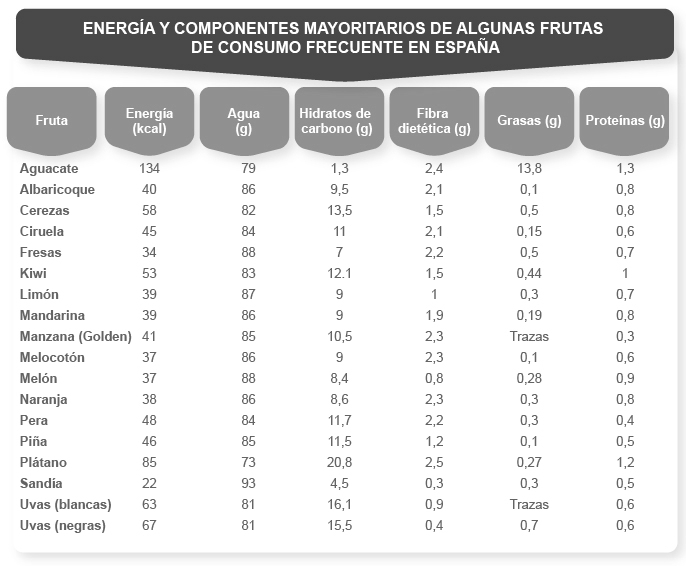
\includegraphics[scale = 0.5]{tablaFrutas} 
\end{figure}	

Algunos de sus pacientes son alérgicos a las frutas de
su lista; digamos que su nuevo paciente no puede 
comer manzanas. La nutrióloga se pregunta si es posible
sustituir los nutrientes aportados por una manzana
con otras frutas de la lista y, si la respuesta es afirmativa,
quisiera dar explícitamente combinaciones de frutas que 
aporten lo mismo que aportaba una cierta cantidad de manzanas
(que no pueden ser incluidas en la dieta del paciente). 
¿Cómo podemos modelar esta situación?

Podemos representar nuestros datos iniciales como
vectores de $\IR^{6}$; por ejemplo, el vector
nutricional de una manzana sería
\[
x_{manzana} = (41, 85, 10.5, 2.3, 0, 0.3)
\in \IR^{6}.
\]
Definamos a $\mathcal{A}$ como el subconjunto de $\IR^{6}$
que consta de todos los vectores fruta,
\[
\mathcal{A} = \{ x_{aguacate}, x_{albaricoque}, \ldots , x_{uvasB},
x_{uvasN} \}.
\]

Nota que, en este contexto, las combinaciones lineales
con coeficientes naturales tienen una interpretación física; por
ejemplo, el vector
\[
2x_{pera} + 5 x_{fresa} + 3 x_{cereza}
\]
representa la información nutrimental de 2 peras,
5 fresas y 3 cerezas (luego, la cantidad de calorías y componentes
que alguien estaría obteniendo al consumir esta cantidad de frutas).

El problema de la nutrióloga queda expresado en términos
de álgebra lineal como sigue:
¿es $x_{manzana}$ elemento del subespacio de $\IR^{6}$ generado
por los vectores $x_{aguacate}, x_{albaricoque}, \ldots ,
x_{uvaB}, x_{uvaN}$? Nota que, implícitamente,
el problema nos permite limitarnos al conjunto de
las combinaciones lineales finitas de los vectores fruta
(menos el vector manzana) y no considerar a todo $\IR^{6}$
(para este problema, no nos interesan vectores que no sean combinaciones
lineales de vectores fruta). La teoría estudiada antes nos asegura que
\begin{itemize}
	\item Tal conjunto de combinaciones de vectores fruta
	es un subespacio de $\IR^{6}$ y,
	\item de hecho, es el menor subespacio de $\IR^{6}$ que contiene 
	a los vectores fruta menos el manzana.
\end{itemize}

La pregunta de la nutrióloga queda entonces expresada en ver si ocurre
\[
x_{manzana} \in \langle \mathcal{A} - \{ x_{manzana} \} \rangle
\]
o no.
\marginnote{No nos interesan todos los elementos de $\IR^{6}$, sino
sólo aquellos que sean combinaciones lineales de vectores fruta;
estamos reemplazando a nuestro espacio de trabajo $\IR^{6}$
por $\langle \mathcal{A} \rangle$.}

Observa que los vectores son mucho más que una forma conveniente de 
almacenar información: podemos hacer operaciones de ellos e
interpretarlas en el contexto del 
problema físico planteado.

Con las definiciones e ideas que planteamos en los siguientes capítulos,
podremos 
\begin{itemize}
	\item Determinar cuándo existen combinaciones de frutas
	que aporten lo mismo que cierta cantidad de manzanas,
	\item Decir si hay una única forma o varias de expresar manzanas
	en términos de combinaciones lineales de frutas específicas
	\item Usar argumentos de dimensionalidad para determinar
	cuándo subconjuntos de frutas son suficientes para
	sustituir a todas las demás
\end{itemize}

Es fácil pensar requerimientos razonables
que complicarían aún más la situación; por ejemplo, considera que,
en un escenario realista, 
\begin{itemize}
	\item Un paciente podría tener no solo posibles alergias
	como limitantes para definir una dieta, sino también 
	un presupuesto mensual al que deba apegarse, presupuesto
	que podría reducir aún más las opciones o cantidades
	de fruta que puede consumir (por ejemplo, esto podría implicar
	que combinaciones lineales que contengan al vector
	$x_{aguacate}$ sólo sean consideradas cuando su coeficiente
	-i.e. el escalar por el que se multiplica a $x_{aguacate}$ - 
	no sea mayor a cierto valor).
\end{itemize}



\begin{figure}[H]
\centering\captionsetup{format = hang}
	\begin{measuredfigure}
		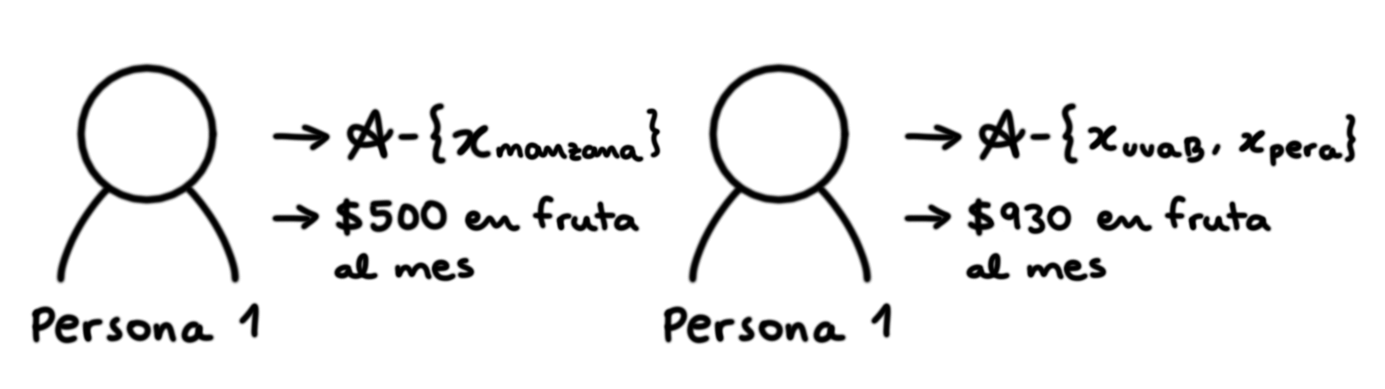
\includegraphics[scale=2]{3} 
		\caption{Cada paciente tiene sus necesidades personales,
		por ejemplo, las frutas a las que es alérgico (o que no le
		gustan, y quiere evitar en su dieta) y su presupuesto mensual.
		Esto cambia el espacio de combinaciones lineales a considerar
		para cada uno, y las combinaciones lineales aceptables.}
 	\end{measuredfigure}
 \end{figure}

Incluso en esta situación tan simplificada, vemos la utilidad
de usar el marco teórico ofrecido por el álgebra lineal para
modelar la situación; con los conocimientos de los próximos
capítulos seremos capaces de resolver los problemas
aquí planteados. 